\section{Introdução}

\begin{frame}{Contextualização}

\begin{columns}[T,onlytextwidth]

\begin{column}{0.42\textwidth}

  \vspace{1.15cm}

  \begin{block}{Modelos clássicos}
    \begin{itemize}
      \item CNNs apresentam excelente desempenho em tarefas de
      classificação de imagens.

      \item Redes pré-treinadas podem extrair representações visuais
      robustas e reutilizáveis.

      \item As características extraídas podem ser fornecidas a diferentes
      classificadores.
    \end{itemize}
  \end{block}
\end{column}

\begin{column}{0.56\textwidth}
  \begin{figure}
  \centering
  \includegraphics[width=0.7\textwidth]{./resources/cifar10.png}
  \caption{Exemplo de imagens do dataset Cifar10.}
  \end{figure} 
\end{column}

\end{columns}
\end{frame}

\begin{frame}{Motivação do estudo}

  \begin{block}{Circuitos quânticos variacionais}
    \begin{itemize}
      \item Codificam dados clássicos em estados quânticos.

      \item Aplicam transformações unitárias parametrizadas, cujos
      parâmetros podem ser ajustados durante o treinamento.
      
      \item Produzem saídas por meio da medição de observáveis quânticos.
    \end{itemize}
  \end{block}
  

  \begin{block}{Abordagem híbrida}
A proposta combina as capacidades complementares dos paradigmas clássico e quântico. Uma CNN pré-treinada extrai representações visuais compactas e robustas, enquanto um circuito quântico variacional atua como classificador sobre essas características. Essa arquitetura híbrida permite investigar se transformações quânticas parametrizadas, baseadas em superposição, interferência e emaranhamento, podem alcançar desempenho competitivo, considerando as limitações atuais de qubits e de profundidade dos circuitos.
\end{block}
  
\end{frame}

%------------------------------------------------
\begin{frame}{Objeto de estudo}

\begin{alertblock}{Desafio experimental}
O desempenho de um classificador quântico depende de diferentes escolhas de
projeto, como:
\begin{itemize}
\item o número de qubits;
\item a estratégia de codificação das características;
\end{itemize}
\end{alertblock}

\vspace{0.1cm}

\begin{center}
\textbf{Essas escolhas devem ser avaliadas de forma controlada e comparadas com um baseline clássico competitivo.}
\end{center}

\end{frame}

%------------------------------------------------
\begin{frame}{Ideia central}

\begin{block}{Proposta}
Avaliar diferentes configurações de classificadores quânticos variacionais,
variando o número de qubits e a estratégia de codificação, e comparar seus
resultados com uma MLP clássica treinada sobre as mesmas características
reduzidas dimensionalmente e sob as mesmas condições experimentais.
\end{block}

\vspace{0.15cm}

\begin{center}
\begin{tikzpicture}[
scale=0.9,
transform shape,
box/.style={
draw,
rounded corners,
align=center,
minimum width=2.05cm,
minimum height=0.75cm,
font=\small
},
arrow/.style={
-{Latex[length=2mm]},
thick
},
node distance=0.35cm and 0.45cm
]

\node[box,fill=SoftGray] (img) {Imagem};

\node[
box,
fill=NeuralOrange!20,
right=of img
] (cnn) {CNN pré-treinada\\extratora};

\node[
box,
fill=NeuralOrange!10,
right=of cnn
] (feat) {Características\\profundas};

\node[
box,
fill=DeepBlue!15,
right=of feat
] (red) {Redução de\\dimensionalidade};

\node[
box,
fill=QuantumPurple!20,
below right=0.15cm and 0.55cm of red
] (vqc) {Circuito quântico\\variacional};

\node[
box,
fill=SoftGray,
above right=0.15cm and 0.55cm of red
] (mlp) {MLP\\clássica};

\coordinate (midout) at ($(vqc.east)!0.5!(mlp.east)$);

\node[
box,
fill=AccentGreen!20,
right=1.0cm of midout
] (cls) {Classe\\predita};

\draw[arrow] (img) -- (cnn);
\draw[arrow] (cnn) -- (feat);
\draw[arrow] (feat) -- (red);
\draw[arrow] (red.east) -- (vqc.west);
\draw[arrow] (red.east) -- (mlp.west);
\draw[arrow] (vqc.east) -- (cls.west);
\draw[arrow] (mlp.east) -- (cls.west);

\node[
font=\scriptsize,
text=QuantumPurple,
above=0.05cm of vqc
] {Variação de qubits e codificação};

\node[
font=\scriptsize,
above=0.05cm of mlp
] {Baseline clássico};

\end{tikzpicture}
\end{center}

\end{frame}

\section{Fundamentação Teórica}

\begin{frame}{Da Física Quântica à Computação Quântica}

\begin{block}{Fenômenos em escala microscópica}
Em escalas extremamente pequenas, partículas como elétrons, átomos e
fótons podem apresentar comportamentos que não aparecem na física
clássica, como superposição, interferência, emaranhamento e resultados probabilísticos na medição.
\end{block}

\begin{block}{Do fenômeno físico ao processador}
Em um processador quântico, sistemas físicos microscópicos são controlados
para representar qubits. Pulsos eletromagnéticos, lasers ou outros
mecanismos físicos são utilizados para preparar estados, aplicar portas
quânticas e realizar medições.
\end{block}

\begin{alertblock}{Ideia central}
A computação quântica consiste em controlar e repetir esses fenômenos de
forma organizada, compondo operações em circuitos para realizar uma tarefa
computacional específica.
\end{alertblock}

\[
\text{preparação}
\;\longrightarrow\;
\text{operações quânticas}
\;\longrightarrow\;
\text{interferência}
\;\longrightarrow\;
\text{medição}
\]

\end{frame}

%------------------------------------------------
\begin{frame}{Qubit: Estado e Medição \cite{nielsen2000quantum}}

\begin{columns}[T,onlytextwidth]

\begin{column}{0.47\textwidth}
  \begin{block}{Do bit ao qubit}
    Um bit clássico assume um estado bem definido:
    \[
      0
      \qquad \text{ou} \qquad
      1.
    \]

    Um qubit, por outro lado, é representado por
    \[
      \ket{\psi}
      =
      \alpha\ket{0}
      +
      \beta\ket{1},
    \]
    com
    \[
      \alpha,\beta\in\mathbb{C},
      \qquad
      |\alpha|^2+|\beta|^2=1.
    \]
  \end{block}
\end{column}

\begin{column}{0.49\textwidth}
  \begin{block}{Medição na base computacional}
    Ao medir o estado $\ket{\psi}$, obtém-se um resultado clássico:
    \[
      P(0)=|\alpha|^2,
      \qquad
      P(1)=|\beta|^2.
    \]

    Após a medição, o estado passa a ser compatível com o resultado
    observado:
    \[
      \ket{0}
      \qquad \text{ou} \qquad
      \ket{1}.
    \]
  \end{block}
\end{column}

\end{columns}

\vspace{0.3cm}

\begin{alertblock}{Amplitudes de probabilidade}
Os coeficientes $\alpha$ e $\beta$ não são probabilidades diretamente.
Eles são amplitudes complexas, enquanto as probabilidades observáveis são
obtidas por seus módulos ao quadrado.
\end{alertblock}

\end{frame}

%------------------------------------------------
\begin{frame}{Superposição e Interferência}

\begin{columns}[T,onlytextwidth]

\begin{column}{0.48\textwidth}
  \begin{block}{Superposição durante a computação}
    Durante a execução de um circuito, portas quânticas transformam as
    amplitudes associadas aos estados da base.

    Assim, o estado pode evoluir como
    \[
      \ket{\psi}
      =
      \sum_i c_i\ket{i},
    \]
    sem que seja necessário medir o sistema a cada operação.
  \end{block}
\end{column}

\begin{column}{0.48\textwidth}
  \begin{block}{Interferência entre amplitudes}
    Como as amplitudes podem possuir sinais e fases diferentes, elas podem
    se combinar:
    \begin{itemize}
      \item \textbf{construtivamente}, reforçando determinados estados;
      \item \textbf{destrutivamente}, reduzindo ou cancelando outros.
    \end{itemize}

    A interferência altera as probabilidades observadas ao final do
    circuito.
  \end{block}
\end{column}

\end{columns}

\vspace{0.3cm}

\begin{alertblock}{Papel nos circuitos quânticos}
O processamento quântico não consiste apenas em manter vários estados em
superposição. As portas controlam amplitudes e fases para produzir padrões
de interferência que influenciam o resultado da medição.
\end{alertblock}

\end{frame}

%------------------------------------------------

\begin{frame}{Sistemas com Múltiplos Qubits}

  \begin{columns}[T,onlytextwidth]

  \begin{column}{0.48\textwidth}

  \begin{block}{Espaço de estados}
  Um sistema com $n$ qubits é descrito por um vetor em um espaço de
  dimensão $2^n$:
  \[
    \ket{\psi}
    =
    \sum_{i=0}^{2^n-1}
    c_i\ket{i},
  \]
  com
  \[
    \sum_{i=0}^{2^n-1}|c_i|^2=1.
  \]

  Cada coeficiente $c_i$ é a amplitude associada a um estado da base
  computacional.
  \end{block}

  \end{column}

  \begin{column}{0.48\textwidth}

  \begin{block}{Composição de qubits}
  O estado conjunto é construído pelo produto tensorial:
  \[
    \ket{\psi_{AB}}
    =
    \ket{\psi_A}\otimes\ket{\psi_B}.
  \]

  Por exemplo:
  \[
    \ket{0}\otimes\ket{1}
    =
    \ket{01}.
  \]
  \end{block}

  \begin{exampleblock}{Exemplo: dois qubits}
  \[
  \ket{\psi}
  =
  c_{00}\ket{00}
  +
  c_{01}\ket{01}
  +
  c_{10}\ket{10}
  +
  c_{11}\ket{11}.
  \]

  Uma medição produz apenas um dos resultados:
  \[
  00,\quad 01,\quad 10,\quad 11.
  \]
  \end{exampleblock}

  \end{column}

  \end{columns}

\end{frame}

%------------------------------------------------
\begin{frame}{Emaranhamento Quântico}

\begin{block}{Estados não separáveis}
Em sistemas com múltiplos qubits, pode ocorrer uma correlação quântica que
não pode ser descrita separando o estado de cada qubit.


Um exemplo é o estado de Bell:
\[
  \ket{\Phi^{+}}
  =
  \frac{1}{\sqrt{2}}
  \left(
    \ket{00}
    +
    \ket{11}
  \right).
\]


\end{block}

\vspace{0.2cm}

\begin{columns}[T,onlytextwidth]


\begin{column}{0.48\textwidth}
  \begin{block}{Interpretação}
    Nesse estado, os resultados possíveis são:
    \[
      P(00)=\frac{1}{2},
      \qquad
      P(11)=\frac{1}{2}.
    \]

    Os resultados $\ket{01}$ e $\ket{10}$ possuem probabilidade nula.
  \end{block}
\end{column}

\begin{column}{0.48\textwidth}
  \begin{block}{Consequência}
    Não é possível escrever o estado como
    \[
      \ket{\psi_A}\otimes\ket{\psi_B}.
    \]

    Portanto, o sistema deve ser descrito globalmente, e não como dois
    qubits independentes.
  \end{block}
\end{column}

\end{columns}

\end{frame}

\begin{frame}{Representação na Esfera de Bloch}

  \begin{columns}[T,onlytextwidth]

  \begin{column}{0.42\textwidth}
  
    \[
  \ket{\psi}
  =
  \cos\left(\frac{\theta}{2}\right)\ket{0}
  +
  e^{i\phi}
  \sin\left(\frac{\theta}{2}\right)\ket{1}
  \]

  \begin{figure}
  \centering
  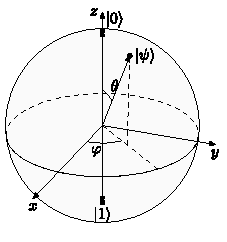
\includegraphics[width=0.7\textwidth]{./resources/Bloch_Sphere_representation.pdf}
  \end{figure}

  \end{column}

  \begin{column}{0.56\textwidth}

  \begin{block}{Interpretação geométrica}
  Para um único qubit, cada estado puro pode ser representado como um ponto
 na superfície da \textbf{esfera de Bloch}. As portas de rotação são dadas por

  \[
  \begin{aligned}
  R_x(\alpha)
  &=
  \begin{pmatrix}
  \cos\left(\frac{\alpha}{2}\right)
  &
  -i\sin\left(\frac{\alpha}{2}\right)
  \\
  -i\sin\left(\frac{\alpha}{2}\right)
  &
  \cos\left(\frac{\alpha}{2}\right)
  \end{pmatrix},
  \\[0.3cm]
  R_y(\beta)
  &=
  \begin{pmatrix}
  \cos\left(\frac{\beta}{2}\right)
  &
  -\sin\left(\frac{\beta}{2}\right)
  \\
  \sin\left(\frac{\beta}{2}\right)
  &
  \cos\left(\frac{\beta}{2}\right)
  \end{pmatrix},
  \\[0.3cm]
  R_z(\gamma)
  &=
  \begin{pmatrix}
  e^{-i\gamma/2} & 0
  \\
  0 & e^{i\gamma/2}
  \end{pmatrix}.
  \end{aligned}
  \]

  Essas operações correspondem a rotações do vetor de estado em torno dos
  eixos $x$, $y$ e $z$, respectivamente.
  \end{block}
  \vspace{0.2cm}

  
  \end{column}
  \end{columns}
\end{frame}

\begin{frame}{Observáveis e Medição Quântica I}

\begin{block}{O que é um observável?}
Um observável é um operador Hermitiano que representa uma quantidade
mensurável do sistema. Para um estado $\ket{\psi}$, sua saída é descrita
pelo valor esperado
\[
  \langle O\rangle
  =
  \bra{\psi}O\ket{\psi},
\]
que corresponde à média dos resultados obtidos em várias execuções do
circuito.
\end{block}

\vspace{0.2cm}

\begin{alertblock}{Por que usar observáveis em aprendizado de máquina?}
Os observáveis convertem o estado quântico em valores clássicos reais,
que podem ser usados como escores de classificação e no cálculo da função
de perda. A escolha do observável determina qual informação do estado
final será extraída.
\end{alertblock}

\end{frame}

\begin{frame}{Observáveis e Medição Quântica II}
\begin{columns}[T,onlytextwidth]

\begin{column}{0.48\textwidth}
\begin{block}{Exemplo: observável $Z$}
\[
  Z=
  \begin{pmatrix}
    1&0\\
    0&-1
  \end{pmatrix}.
\]

Seus resultados possíveis são
\[
  \ket{0}\rightarrow +1,
  \qquad
  \ket{1}\rightarrow -1.
\]

Assim,
\[
  \langle Z\rangle
  =
  P(0)-P(1)
  \in[-1,1].
\]
\end{block}
\end{column}

\begin{column}{0.48\textwidth}
\begin{block}{Sistemas com vários qubits}
Para medir o qubit $j$, utiliza-se
\[
  Z_j
  =
  I^{\otimes(j-1)}
  \otimes Z
  \otimes I^{\otimes(n-j)}.
\]

Podem ser obtidas saídas locais,
\[
  \langle Z_1\rangle,\ldots,\langle Z_n\rangle,
\]
ou correlações, como
\[
  \langle Z_1Z_2\rangle.
\]
\end{block}
\end{column}

\end{columns}

\end{frame}

\begin{frame}{Redução de Dimensionalidade com PCA}

\begin{block}{O que é PCA?}
A Análise de Componentes Principais (\textit{Principal Component Analysis})
é uma técnica linear de redução de dimensionalidade que transforma um vetor
de características em um novo conjunto de variáveis não correlacionadas,
chamadas de \textbf{componentes principais}.
\end{block}

\begin{block}{Ideia principal}
As componentes são ordenadas de acordo com a quantidade de variância dos
dados que explicam:
\[
\mathbf{x}\in\mathbb{R}^{d}
\;\longrightarrow\;
\mathbf{z}\in\mathbb{R}^{k},
\qquad k<d.
\]

As primeiras componentes preservam as direções de maior variação do
conjunto de dados.
\end{block}

\begin{alertblock}{Papel no modelo híbrido}
A ResNet18 produz um vetor de características de alta dimensão. O PCA
reduz esse vetor para uma dimensão compatível com a codificação quântica,
buscando preservar a informação mais relevante antes da entrada no circuito.
\end{alertblock}

\end{frame}

\section{Metodologia}

\begin{frame}{Pipeline de Referência: Classificador Clássico}
  \begin{center}
  \begin{tikzpicture}[
      box/.style={
        draw,
        rounded corners,
        align=center,
        minimum width=2.05cm,
        minimum height=0.9cm
      },
      arrow/.style={-{Latex[length=2mm]},thick}
    ]
    \node[box,fill=SoftGray] (img) {Imagem\\CIFAR-10};
    \node[box,fill=NeuralOrange!20,right=0.25cm of img] (resnet)
      {ResNet18\\pré-treinada};
    \node[box,fill=NeuralOrange!10,right=0.25cm of resnet] (feat)
      {Vetor de\\características};
    \node[box,fill=DeepBlue!10,right=0.25cm of feat] (proj)
      {Redução\\dimensional};
    \node[box,fill=DeepBlue!20,right=0.25cm of proj] (mlp)
      {MLP\\clássica};
    \node[box,fill=AccentGreen!20,right=0.25cm of mlp] (class)
      {Classe\\predita};

    \draw[arrow] (img) -- (resnet);
    \draw[arrow] (resnet) -- (feat);
    \draw[arrow] (feat) -- (proj);
    \draw[arrow] (proj) -- (mlp);
    \draw[arrow] (mlp) -- (class);
  \end{tikzpicture}
  \end{center}

  \vspace{0.3cm}

  \begin{block}{Baseline experimental}
    O desempenho da MLP será utilizado como referência para avaliar a
    competitividade dos classificadores quânticos. Para garantir uma comparação justa, os modelos clássico e quântico receberão as mesmas características extraídas pela ResNet18 escolhida como extratora de características. Além disso, esse modelo também será treinado recebendo a mesma quantidade de features que os modelos híbridos.
  \end{block}
\end{frame}

\begin{frame}[fragile]{Arquitetura da MLP Clássica}

\begin{lstlisting}[style=pythonstyle]
class MLPClassifier(nn.Module):
    def __init__(self, input_dim, config):
        super().__init__()

        self.network = _build_mlp(
            input_dim,
            config.get("hidden_layers", [256]),
            config.get("dropout", 0.3),
            config["num_classes"],
        )

    def forward(self, features):
        return self.network(features)
\end{lstlisting}

\begin{block}{Estrutura utilizada}
A MLP recebe as características extraídas pela CNN e aplica uma ou mais
camadas densas. Na configuração padrão, utiliza-se uma camada oculta com
$256$ neurônios, \textit{dropout} de $0{,}3$ e uma camada de saída com um
neurônio para cada classe.
\end{block}

\end{frame}

\begin{frame}[shrink=15]{Pipeline Proposto: Classificador Quântico}
  \begin{center}
  \begin{tikzpicture}[
      box/.style={
        scale=0.85,
        draw,
        rounded corners,
        align=center,
        minimum width=2.05cm,
        minimum height=0.9cm
      },
      arrow/.style={-{Latex[length=2mm]},thick}
    ]
    \node[box,fill=SoftGray] (img) {Imagem\\CIFAR-10};
    \node[box,fill=NeuralOrange!20,right=0.3cm of img] (cnn)
      {ResNet18\\pré-treinada};
    \node[box,fill=NeuralOrange!10,right=0.3cm of cnn] (proj)
      {Redução\\dimensional};
    \node[box,fill=QuantumPurple!15,right=0.3cm of proj] (encode)
      {Codificação\\quântica};
    \node[box,fill=QuantumPurple!25,right=0.3cm of encode] (vqc)
      {Circuito quântico\\variacional};
    \node[box,fill=AccentGreen!20,right=0.3cm of vqc] (out)
      {Medição};
    \node[box,fill=AccentGreen!20,right=0.3cm of out] (linear)
      {Linear};
    \node[box,fill=AccentGreen!20,right=0.3cm of linear] (pred)
      {Predição};

    \draw[arrow] (img) -- (cnn);
    \draw[arrow] (cnn) -- (proj);
    \draw[arrow] (proj) -- (encode);
    \draw[arrow] (encode) -- (vqc);
    \draw[arrow] (vqc) -- (out);
    \draw[arrow] (out) -- (linear);
    \draw[arrow] (linear) -- (pred);
  \end{tikzpicture}
  \end{center}

  \vspace{0.25cm}

  \begin{columns}[T,onlytextwidth]
    \begin{column}{0.48\textwidth}
      \begin{block}{Etapa clássica}
        A ResNet18 extrai representações visuais das imagens, enquanto a redução
        dimensional ajusta o vetor de características à quantidade de informações
        que pode ser codificada pelo circuito quântico.
      \end{block}
    \end{column}

    \begin{column}{0.48\textwidth}
      \begin{block}{Etapa quântica}
        O vetor reduzido é codificado em um estado quântico e processado por
        camadas parametrizadas. As medições realizadas ao final do circuito são
        utilizadas para produzir a predição da classe \cite{amadoun2026evaluation,cerezo2021variational}.
      \end{block}
    \end{column}
  \end{columns}

  \vspace{0.2cm}

  \begin{alertblock}{Ambiente de execução}
    Os circuitos quânticos serão executados em simuladores, permitindo avaliar diferentes configurações de qubits e estratégias de codificação em um ambiente controlado e livre de ruídos de hardware.
  \end{alertblock}
\end{frame}


%------------------------------------------------
\begin{frame}[shrink=15]{Codificação de Dados em Estados Quânticos}

  \begin{alertblock}{Interpretação para aprendizado de máquina}
    Antes de serem consumidos pelos circuitos quânticos variacionais, os dados clássicos devem ser transformados em operações ou amplitudes
    compatíveis com um estado quântico. Esse processo é denominado
    \highlight{codificação dos dados}.
  \end{alertblock}
  
  \begin{columns}[T,onlytextwidth]

    \begin{column}{0.48\textwidth}
      \begin{block}{Angle encoding}
        Cada característica controla o ângulo de uma porta de rotação:
        \[
          \ket{\psi(\mathbf{x})}
          =
          \bigotimes_{i=1}^{n}
          R_y(x_i)\ket{0}.
        \]

        \begin{itemize}
          \item Implementação simples;
          \item Baixa profundidade;
          \item Em geral, uma característica por qubit e por camada.
        \end{itemize}
      \end{block}
    \end{column}

    \begin{column}{0.48\textwidth}
      \begin{block}{Amplitude encoding}
        As características são inseridas nas amplitudes do estado:
        \[
          \ket{\psi(\mathbf{x})}
          =
          \sum_{i=0}^{2^n-1} x_i\ket{i}.
        \]

        \begin{itemize}
          \item Codifica até $2^n$ valores;
          \item Requer normalização;
          \item A preparação do estado pode ser custosa.
        \end{itemize}
      \end{block}
    \end{column}
  \end{columns}
\end{frame}


%------------------------------------------------
\begin{frame}[shrink=12]{Circuito Quântico Variacional}

\begin{columns}[T,onlytextwidth]

\begin{column}{0.48\textwidth}
\vspace{0.65cm}
\begin{block}{Fluxo do circuito}
Dado um vetor de características $\mathbf{x}$, o circuito realiza:

\begin{enumerate}
  \item codificação dos dados nos $n$ qubits;
  \item aplicação de rotações parametrizadas;
  \item criação de correlações por portas CNOT;
  \item medição do observável $Z$ em cada qubit.
\end{enumerate}

O estado final é dado por
\[
  \ket{\psi(\mathbf{x},\boldsymbol{\theta})}
  =
  U_{\mathrm{var}}(\boldsymbol{\theta})
  U_{\mathrm{enc}}(\mathbf{x})
  \ket{0}^{\otimes n}.
\]
\end{block}

\end{column}

\begin{column}{0.48\textwidth}

\begin{block}{Ansatz variacional}
Cada camada aplica, em cada qubit,
\[
  R_x(\theta_{\ell,i,1}),
  \qquad
  R_y(\theta_{\ell,i,2}),
  \qquad
  R_z(\theta_{\ell,i,3}),
\]
seguida de portas CNOT entre qubits vizinhos.

A transformação de uma camada pode ser representada por
\[
  U^{(\ell)}
  =
  U_{\mathrm{ent}}
  \prod_{i=1}^{n}
  R_z(\theta_{\ell,i,3})
  R_y(\theta_{\ell,i,2})
  R_x(\theta_{\ell,i,1}).
\]

O bloco é repetido por $L$ camadas:
\[
  U_{\mathrm{var}}
  =
  U^{(L)}\cdots U^{(2)}U^{(1)}.
\]
\end{block}


\end{column}

\end{columns}

\end{frame}

\begin{frame}[shrink=15]{Circuito Quântico Variacional}
  
  \vspace{1.5cm}

  \begin{columns}[T,onlytextwidth]

    \begin{column}{0.48\textwidth}
      \begin{block}{Saída quântica}
      Para cada qubit $j$, calcula-se
      \[
        z_j
        =
        \bra{\psi(\mathbf{x},\boldsymbol{\theta})}
        Z_j
        \ket{\psi(\mathbf{x},\boldsymbol{\theta})},
      \]
      produzindo o vetor
      \[
        \mathbf{z}
        =
        \big[
          \langle Z_1\rangle,
          \ldots,
          \langle Z_n\rangle
        \big]
        \in[-1,1]^n.
      \]
      \end{block}
    \end{column}

    \begin{column}{0.48\textwidth}
      \begin{alertblock}{Classificação híbrida}
      O vetor de medições não representa diretamente as classes. Uma camada
      linear clássica realiza
      \[
        \mathbf{o}
        =
        W\mathbf{z}+\mathbf{b},
      \]
      gerando um logit para cada classe. Os parâmetros do circuito e da camada
      linear são treinados conjuntamente por retropropagação.
      \end{alertblock}

    \end{column}

  \end{columns}
\end{frame}


\begin{frame}[shrink=15]{Ilustração do Circuito Quântico Variacional}

\vspace{1.5cm}
  
\centering
\begin{quantikz}[row sep=0.35cm, column sep=0.22cm]
\lstick{$\ket{0}$} 
  & \gate{R_y(x_1)} 
  & \slice{$\text{Camada } \ell$}
  & \gate{R_x(\theta_{\ell,1,1})}
  & \gate{R_y(\theta_{\ell,1,2})}
  & \gate{R_z(\theta_{\ell,1,3})}
  & \ctrl{1}
  & \qw
  & \push{\cdots}
  \slice{}
  & \meter{}
  & \rstick{$\langle Z_1\rangle$} \\
\lstick{$\ket{0}$} 
  & \gate{R_y(x_2)} 
  & 
  & \gate{R_x(\theta_{\ell,2,1})}
  & \gate{R_y(\theta_{\ell,2,2})}
  & \gate{R_z(\theta_{\ell,2,3})}
  & \targ{}
  & \ctrl{1}
  & \push{\cdots}
  & \meter{} 
  & \rstick{$\langle Z_2\rangle$} \\
\lstick{$\vdots$} 
  & \vdots 
  & 
  & \vdots
  & \vdots
  & \vdots
  & \vdots
  & \vdots
  & 
  & \vdots
  & \rstick{$\vdots$} \\
\lstick{$\ket{0}$} 
  & \gate{R_y(x_n)} 
  & 
  & \gate{R_x(\theta_{\ell,n,1})}
  & \gate{R_y(\theta_{\ell,n,2})}
  & \gate{R_z(\theta_{\ell,n,3})}
  & \qw
  & \targ{}
  & \push{\cdots}
  & \meter{} 
  & \rstick{$\langle Z_n\rangle$}
\end{quantikz}

\end{frame}


\begin{frame}{Papel das rotações no circuito quântico}

\begin{columns}[T,onlytextwidth]

\begin{column}{0.48\textwidth}

\begin{block}{Rotações parametrizadas}
Após a codificação, portas como
\[
R_x(\theta),\quad R_y(\theta),\quad R_z(\theta)
\]
transformam o estado quântico.

Durante o treinamento, seus ângulos são ajustados para produzir medições
mais adequadas à tarefa de classificação.
\end{block}

\begin{alertblock}{Intuição para classificação}
O treinamento busca levar amostras de classes diferentes a estados que
produzam valores de medição mais distintos.
\end{alertblock}

\end{column}

\begin{column}{0.48\textwidth}

\begin{block}{Emaranhamento}
Portas como CNOT e CZ criam correlações entre os qubits, permitindo que o
circuito processe conjuntamente diferentes características dos dados.
\end{block}

\begin{alertblock}{Saída do circuito}
A medição de observáveis, como $Z$, produz valores em $[-1,1]$ utilizados na classificação. Como cada execução fornece apenas uma amostra, o circuito é repetido por vários \textit{shots} para estimar o valor esperado.

\end{alertblock}

\end{column}

\end{columns}

\end{frame}


%------------------------------------------------
\begin{frame}[shrink=20]{Treinamento do Modelo Híbrido}

\begin{block}{Fluxo de otimização}
O circuito produz valores esperados que são enviados às camadas clássicas:
\[
\mathbf{x}
\longrightarrow
f_{\boldsymbol{\theta}}(\mathbf{x})
\longrightarrow
\mathcal{L}.
\]

A função de perda é calculada classicamente, e um otimizador atualiza tanto
os parâmetros quânticos quanto os parâmetros clássicos:
\[
\boldsymbol{\theta}
\leftarrow
\boldsymbol{\theta}
-
\eta\nabla_{\boldsymbol{\theta}}\mathcal{L}.
\]
\end{block}

\begin{block}{Regra \textit{parameter-shift}}
Para portas de rotação parametrizadas, o gradiente pode ser obtido
avaliando o circuito em dois valores deslocados do parâmetro:
\[
\frac{\partial f}{\partial \theta}
=
\frac{1}{2}
\left[
f\left(\theta+\frac{\pi}{2}\right)
-
f\left(\theta-\frac{\pi}{2}\right)
\right].
\]

Assim, não é necessário acessar diretamente o estado interno do hardware:
o gradiente é estimado a partir de novas execuções do circuito.
\end{block}

\begin{alertblock}{Custo computacional}
Para cada parâmetro treinável, a regra básica exige duas avaliações
adicionais do circuito. Com $P$ parâmetros, um passo de gradiente pode
exigir aproximadamente $2P$ execuções, além da avaliação original.
\end{alertblock}

\end{frame}

\begin{frame}[shrink=10]{Diferenciação e Execução das Camadas Quânticas}

\begin{block}{Por que a retropropagação clássica não é aplicada diretamente?}
Em uma rede neural clássica, os valores intermediários das camadas são
armazenados e reutilizados no cálculo dos gradientes.

Em um computador quântico real:
\begin{itemize}
  \item as amplitudes do estado não podem ser lidas diretamente;
  \item a medição altera o estado quântico;
  \item o hardware retorna apenas amostras ou valores esperados;
  \item não há acesso clássico aos estados intermediários do circuito.
\end{itemize}

Por isso, os gradientes são obtidos por novas execuções do circuito,
utilizando métodos como \textit{parameter-shift} \cite{bergholm2018pennylane}.
\end{block}

\begin{alertblock}{Hardware quântico versus simulador}
\begin{itemize}
  \item \textbf{Hardware real:} o circuito é executado no processador
  quântico e os gradientes dependem de medições repetidas.

  \item \textbf{Simulador:} o estado pode ser armazenado numericamente,
  permitindo métodos como diferenciação por estado, método adjunto e,
  em alguns casos, aceleração por GPU.
\end{itemize}
\end{alertblock}

\end{frame}

\begin{frame}[shrink=15]{Treinamento da Rede Híbrida}

\begin{algorithm}[H]
\small

\KwIn{
Dados $\mathcal{D}$, ResNet18 pré-treinada, $n$ qubits,
$L$ camadas e $E$ épocas
}

\KwOut{
Parâmetros treinados $\boldsymbol{\theta}$, $W$ e $b$
}

Congelar o extrator ResNet18\;

Inicializar $\boldsymbol{\theta}$, $W$ e $b$\;

\For{$e \leftarrow 1$ \KwTo $E$}{

  \For{cada lote $(\mathbf{I},\mathbf{y})$}{

    $\mathbf{h}
    \leftarrow
    \operatorname{ResNet18}(\mathbf{I})$\;

    $\mathbf{x}
    \leftarrow
    \operatorname{PCA/Projeção}(\mathbf{h})$\;

    \For{cada amostra $\mathbf{x}_k$}{

      $\ket{\psi_k}
      \leftarrow
      U_{\mathrm{enc}}(\mathbf{x}_k)
      \ket{0}^{\otimes n}$\;

      \For{$\ell \leftarrow 1$ \KwTo $L$}{

        Aplicar $R_x$, $R_y$ e $R_z$ parametrizadas em cada qubit\;

        Aplicar CNOTs entre qubits vizinhos\;
      }

      $\mathbf{z}_k
      \leftarrow
      [
      \langle Z_1\rangle,
      \ldots,
      \langle Z_n\rangle
      ]$\;
    }

    $\mathbf{o}\leftarrow W\mathbf{z}+b$\;

    $\mathcal{L}
    \leftarrow
    \operatorname{CrossEntropy}(\mathbf{o},\mathbf{y})$\;

    Calcular gradientes clássicos por retropropagação\;

    Calcular gradientes quânticos por \textit{parameter-shift}\;

    Atualizar $\boldsymbol{\theta}$, $W$ e $b$\;
  }
}

\caption{Fluxo de treinamento do modelo híbrido.}
\end{algorithm}

\end{frame}


\begin{frame}{O que será analisado?}

\begin{block}{A estratégia de codificação influencia o desempenho}
Mesmo com o extrator clássico mantido fixo, diferentes formas de codificar
as características no circuito podem produzir resultados distintos:
\textit{Angle Encoding}
e
\textit{Amplitude Encoding}.
\end{block}

\begin{block}{Mais qubits não implica necessariamente melhor desempenho}
O aumento do número de qubits amplia o espaço de estados e a capacidade
de representação do circuito, mas também pode elevar o custo computacional
e dificultar a otimização.

Serão avaliadas configurações com:
\[
4,\qquad 6 \qquad \text{e} \qquad 8 \text{ qubits}.
\]
\end{block}

\begin{block}{O modelo híbrido pode ser competitivo}
Um classificador quântico variacional pode apresentar desempenho competitivo
em relação a uma MLP clássica, especialmente quando recebe características
visuais compactas e informativas extraídas por uma CNN pré-treinada.
\end{block}

\end{frame}

\begin{frame}{Configurações de Treinamento}

\begin{columns}[T,onlytextwidth]

\begin{column}{0.48\textwidth}

\begin{block}{Dados, pré-processamento e rede}
\begin{itemize}
  \item Dataset: CIFAR-10 ($32\times32$)
  \item Imagens redimensionadas para $224\times224$
  \item Divisão:
  \[
    70\% \text{ treino},\quad
    15\% \text{ validação},\quad
    15\% \text{ teste}
  \]
  \item Tamanho do lote: $64$
  \item Aumentos de dados:
  \begin{itemize}
    \item recorte aleatório;
    \item \textit{color jitter} de $0{,}1$.
  \end{itemize}

  \item ResNet18 pré-treinada na ImageNet
  \item Pesos do extrator congelados
  \item Redução de dimensionalidade por PCA

\end{itemize}
\end{block}

\end{column}

\begin{column}{0.48\textwidth}

\begin{block}{Otimização}
\begin{itemize}
  \item Otimizador Adam
  \item Taxa de aprendizado:
  \[
    10^{-4}
  \]
  \item \textit{Weight decay}:
  \[
    10^{-4}
  \]
  \item Máximo de $500$ épocas
  \item Agendador cossenoidal
  \item \textit{Early stopping} com paciência de $8$ épocas
  \item Lote quântico: $16$
\end{itemize}
\end{block}

\end{column}

\end{columns}

\end{frame}

\section{Resultados Parciais}

\begin{frame}{Resultados I}
  \begin{table}[ht]
\centering
\small
\setlength{\tabcolsep}{6pt}
\renewcommand{\arraystretch}{1.15}

\begin{tabular}{lllrrr}
\toprule
Redução
& Codificação
& Qubits
& Parâmetros
& Acurácia
& Tempo (min) \\
\midrule

\rowcolor{red!20}
PCA para 4
& angle
& 4
& 74
& \textbf{0.2584}
& 115.82 \\

PCA para 6
& angle
& 6
& 106
& 0.2781
& 462.62 \\

PCA para 8
& angle
& 8
& 138
& 0.3280
& 245.46 \\

PCA para 16
& amplitude
& 4
& 74
& 0.3976
& 99.09 \\

\rowcolor{green!20}
PCA para 64
& amplitude
& 6
& 106
& \textbf{0.4233}
& 127.79 \\

PCA para 256
& amplitude
& 8
& 138
& 0.3941
& 542.99 \\

\bottomrule
\end{tabular}

\caption{
Resultados das configurações híbridas avaliadas, variando a estratégia
de codificação e o número de qubits. O melhor resultado está destacado
em verde e o pior em vermelho.
}
\label{tab:resultados_hibridos}
\end{table}
\end{frame}

\begin{frame}{Resultados II}
  \begin{table}[ht]
\centering
\scriptsize
\setlength{\tabcolsep}{3.5pt}
\renewcommand{\arraystretch}{1.12}

\begin{tabular}{lllllrrr}
\toprule
Modelo
& Features
& Redução
& Codificação
& Qubits
& Parâmetros
& Acurácia
& Tempo (min) \\
\midrule

MLP
& raw
& Sem redução
& --
& --
& 133\,898
& 0.8711
& 0.31 \\

MLP
& PCA
& PCA para 4
& --
& --
& 3\,850
& 0.5540
& 0.28 \\

\rowcolor{red!20}
Híbrido
& PCA
& PCA para 4
& angle
& 4
& 74
& \textbf{0.2584}
& 115.82 \\

MLP
& PCA
& PCA para 6
& --
& --
& 4\,362
& 0.6428
& 0.21 \\

Híbrido
& PCA
& PCA para 6
& angle
& 6
& 106
& 0.2781
& 462.62 \\

MLP
& PCA
& PCA para 8
& --
& --
& 4\,874
& 0.7043
& 0.29 \\

Híbrido
& PCA
& PCA para 8
& angle
& 8
& 138
& 0.3280
& 245.46 \\

MLP
& PCA
& PCA para 16
& --
& --
& 6\,922
& 0.7855
& 0.51 \\

Híbrido
& PCA
& PCA para 16
& amplitude
& 4
& 74
& 0.3976
& 99.09 \\

MLP
& PCA
& PCA para 64
& --
& --
& 19\,210
& 0.8619
& 0.77 \\

\rowcolor{yellow!25}
Híbrido
& PCA
& PCA para 64
& amplitude
& 6
& 106
& \textbf{0.4233}
& 127.79 \\

\rowcolor{green!20}
MLP
& PCA
& PCA para 256
& --
& --
& 68\,362
& \textbf{0.8740}
& 0.44 \\

Híbrido
& PCA
& PCA para 256
& amplitude
& 8
& 138
& 0.3941
& 542.99 \\

\bottomrule
\end{tabular}

\caption{
Comparação entre os classificadores clássicos e híbridos em termos de
dimensionalidade de entrada, número de parâmetros treináveis, acurácia no conjunto de teste e tempo de treinamento.
}
\label{tab:resultados_classificadores}
\end{table}
\end{frame}

\begin{frame}{Evolução da loss}
  \begin{figure}
  \centering
  \includegraphics[width=0.7\textwidth]{./resources/loss_validation_comparison.png}
  \caption{Evolução das funções custo no conjunto de validação.}
  \end{figure}
\end{frame}

\begin{frame}{Síntese dos Resultados}

\begin{itemize}
  \item A MLP clássica apresentou o melhor desempenho geral.

  \item A codificação por amplitude superou a codificação angular
  entre os modelos híbridos avaliados.

  \item O aumento do número de qubits não produziu ganhos monotônicos.

  \item Os classificadores híbridos utilizaram poucos parâmetros
  treináveis, mas apresentaram custo de treinamento substancialmente maior.

  \item O melhor modelo híbrido utilizou amplitude encoding e 6 qubits,
  alcançando acurácia de $0.4233$.
\end{itemize}

\end{frame}